\chapter{Metodologia}
em andamento  
 
Neste capítulo, detalhamos os três módulos propostos na Figura \ref{fig:proposta}: 
Condições Iniciais, Treinamento e Geração de Sequências. 
Além disso, apresentamos os métodos de avaliação das proteínas geradas, 
bem como as especificações de hardware e software utilizados.  

\section{Condições Iniciais}

O objetivo do primeiro módulo (Figura \ref{fig:cond_iniciais}) é obter a sequência inicial de aminoácidos e calcular o erro inicial. 
A sequência inicial é gerada passando a estrutura alvo como entrada do \textit{ProteinMPNN}, 
enquanto o erro inicial é definido por:  

\begin{equation}
    Er_{0} = 1 - TMScore(E_{FIX}, E_{ini})
\end{equation}

\noindent
onde $E_{FIX}$ representa a estrutura do fator IX de coagulação (alvo), e $E_{ini}$ é a estrutura correspondente à sequência inicial, predita pelo \textit{ESMFold}. O \textit{TMScore} mede a similaridade entre as estruturas, conforme descrito em \ref{subsection:TMScore}.  
 
\begin{algorithm}
    \caption{Obtenção das Condições Iniciais}
    \label{alg:initial_conditions}
    \begin{algorithmic}[1]
    \Require Estrutura alvo $E_{FIX}$
    \Ensure Sequência inicial $S_{ini}$ e erro inicial $Er_{0}$
    \State $S_{ini} \gets \textit{ProteinMPNN}(E_{FIX})$
    \State $E_{ini} \gets \textit{ESMFold}(S_{ini})$
    \State $Er_{0} \gets 1 - \textit{TMScore}(E_{FIX}, E_{ini})$
    \Return $S_{ini}, Er_{0}$
    \end{algorithmic}
    \end{algorithm}
    
\section{Treinamento}
O módulo de Treinamento consiste em duas etapas: 
**Estágio I** e **Estágio II**, 
detalhados em \ref{subsection:stage1} e \ref{subsection:stage2}, respectivamente. 
Em ambos os estágios, o treinamento ocorre por meio da interação 
entre um **Ambiente de Aprendizado** e um **Agente de Aprendizado**.

\begin{figure}[H]
    \centering
    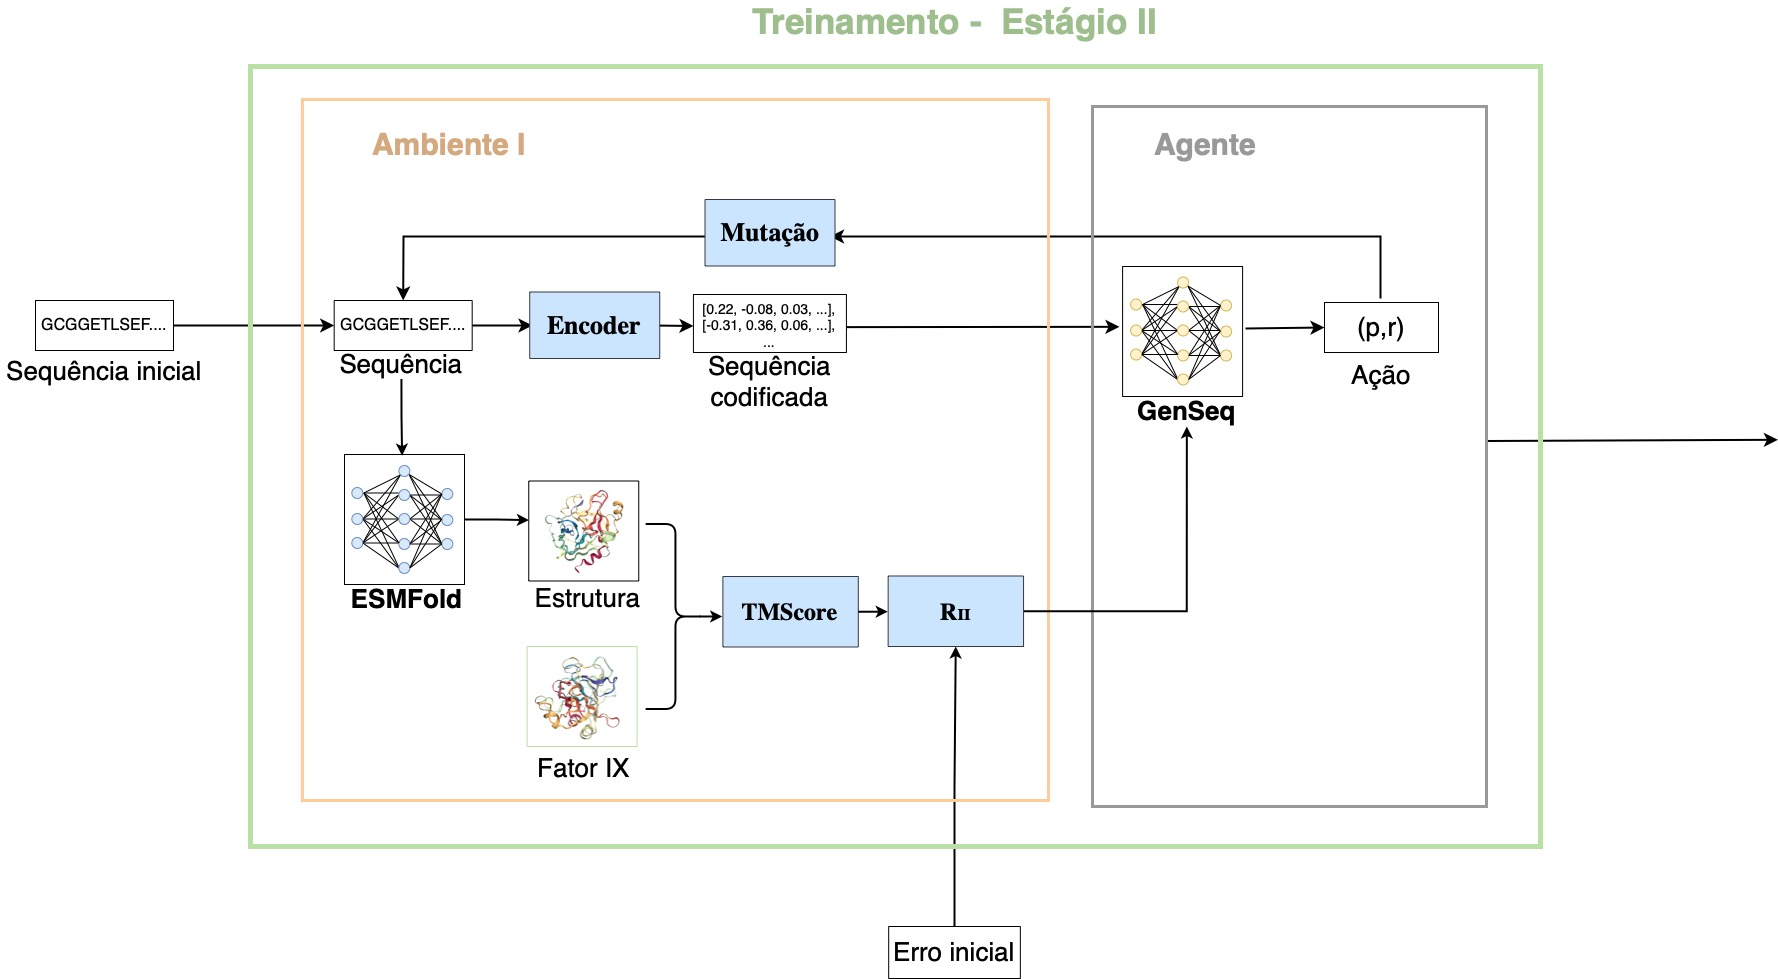
\includegraphics[width=.8\textwidth]{figuras/metodologia-Training.jpg}
    \caption{Fluxo de treinamento do agente GenSeq.}
    \label{fig:training}
\end{figure}

O ambiente de aprendizado é modelado como um **Processo de Decisão de Markov (MDP)**,
 onde o agente aprende a modificar sequências proteicas por meio de mutações direcionadas.
  Durante o treinamento, o agente recebe uma sequência inicial e aprende a otimizá-la por meio 
  de mutações que minimizam o erro estrutural em relação à estrutura alvo. A
   métrica utilizada para avaliar a similaridade estrutural é o **TMScore**.

\begin{algorithm}
    \caption{Treinamento do Agente GenSeq (PPO)}
    \label{alg:train_agent}
    \begin{algorithmic}[1]
    \Require Número de episódios $N$, número máximo de mutações por episódio $M$
    \Ensure Agente treinado $A$
    \State Inicializar agente $A$
    \For{$i = 1$ to $N$}
        \State $S_{t} \gets S_{ini}$  \Comment{Obter sequência inicial}
        \For{$j = 1$ to $M$}
            \State $a_{t} \gets A.\textit{escolher\_ação}(S_{t})$  \Comment{Selecionar mutação}
            \State $S_{t+1} \gets \textit{Aplicar\_Mutação}(S_{t}, a_{t})$
            \State $Er_{t+1} \gets 1 - \textit{TMScore}(E_{FIX}, E_{t+1})$
            \State $R_{t} \gets \textit{Calcular\_Recompensa}(Er_{t}, Er_{t+1})$
            \State $A.\textit{Atualizar\_Política}(S_{t}, a_{t}, R_{t}, S_{t+1})$
            \If{\textit{Critério de Parada Atingido}}
                \State \textbf{break}
            \EndIf
        \EndFor
    \EndFor
    \Return $A$
    \end{algorithmic}
\end{algorithm}

\textbf{Parâmetros do Treinamento}
\begin{enumerate}
    \item \textbf{Número máximo de mutações por episódio}: 45
    \item \textbf{Erro mínimo no episódio}: 0.05
    \item \textbf{Erro máximo no episódio}: 0.083
    \item \textbf{Número de iterações}: 60.000
    \item \textbf{Hiperparâmetros PPO}: $a = 12$, $b = 200$, $c = 50$
    \item \textbf{Número máximo de repetições de aminoácidos em um episódio ($N_{rep}$)}: 7
\end{enumerate}









\subsection{Treinamento - Estágio I}
\label{subsection:stage1}

O primeiro estágio de treinamento tem como objetivo restringir o espaço de busca do Agente, 
incentivando-o a explorar apenas regiões da sequência onde há maior probabilidade de encontrar mutações benéficas.
Para isso, foram aplicadas penalizações às mutações em regiões altamente conservadas 
e àquelas que substituem aminoácidos por resíduos muito distintos em termos de propriedades físico-químicas.
 A função de recompensa utilizada neste estágio é definida como:

\begin{equation}
    R_{I} = -(CS(p) + AminoDist(r, r_{prev}))
\end{equation}

\noindent
Onde:
\begin{itemize}
    \item $p$ é a posição da mutação;
    \item $r$ é o aminoácido inserido na posição $p$;
    \item $r_{prev}$ é o aminoácido original antes da mutação;
    \item $CS(p)$ representa o \textit{Conservation Score} normalizado da posição $p$;
    \item $AminoDist(r, r_{prev})$ é a similaridade entre os aminoácidos $r$ e $r_{prev}$, baseada na matriz de distâncias de \cite{aminodist}.
\end{itemize}

A estratégia geral do treinamento consiste em iniciar com uma sequência inicial 
e aplicar mutações iterativamente, 
utilizando a política aprendida pelo agente. 
O treinamento segue os seguintes passos:

\begin{algorithm}
  \caption{Treinamento - Estágio I}
  \label{alg:train_stage1}
  \begin{algorithmic}[1]
  \Require Número total de iterações $N_{iter}$, número máximo de mutações por episódio $M_{max}$
  \Ensure Agente pré-treinado $A$
  \State Inicializar pesos do agente $A$ aleatoriamente
  \For{$i = 1$ to $N_{iter}$}
      \State $S_{t} \gets S_{ini}$ \Comment{Obter sequência inicial}
      \State $P_{val} \gets \textit{Todas as posições na sequência}$
      \State $R_{val} \gets \textit{Todos os aminoácidos}$
      \For{$j = 1$ to $M_{max}$}
          \State $a_{t} \gets A.\textit{escolher\_ação}(S_{t})$
          \State $S_{t+1} \gets \textit{Aplicar\_Mutação}(S_{t}, a_{t})$
          \State $R_{I} \gets -(CS(p) + AminoDist(r, r_{prev}))$
          \State Atualizar política do agente com PPO
          \If{$p \in P_{val}$}
              \State Remover $p$ de $P_{val}$
          \EndIf
          \If{$r$ já foi escolhido $N_{rep}$ vezes}
              \State Remover $r$ de $R_{val}$
          \EndIf
          \If{Critério de parada atingido}
              \State \textbf{break}
          \EndIf
      \EndFor
  \EndFor
  \Return $A$
  \end{algorithmic}
\end{algorithm}

Após o término do primeiro estágio de treinamento, o agente é avaliado contra uma política de mutações aleatórias para verificar sua eficácia. Os resultados mostram que a distribuição de recompensas do agente é significativamente superior à de um agente aleatório (Figura \ref{fig:box-pre-train}).

\begin{figure}[H]
  \centering
  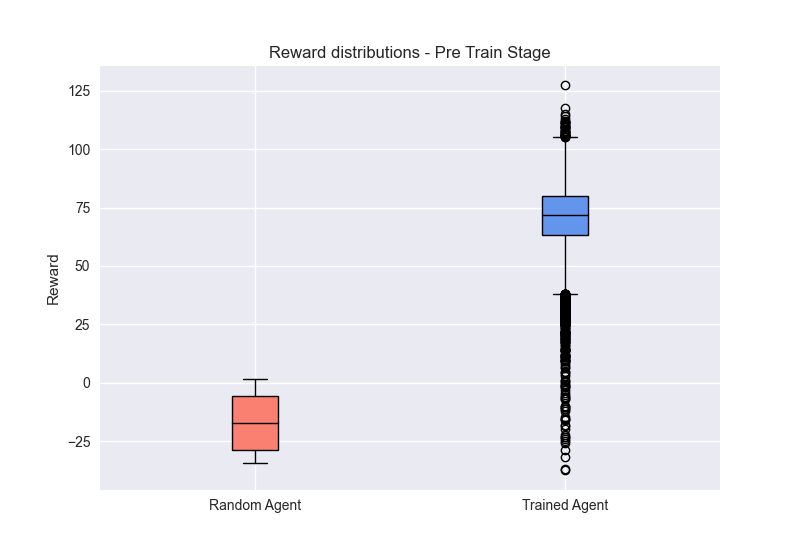
\includegraphics[width=.8\linewidth]{figuras/plot_box_pre_train_reward.jpg}  
  \caption{Comparação do Agente pré-treinado com um Agente aleatório.}
  \label{fig:box-pre-train}
\end{figure}

O comportamento do agente durante o treinamento pode ser visualizado na Figura \ref{fig:rew_per_ep_pretrain}, onde a média móvel das recompensas por episódio estabiliza após aproximadamente 2500 episódios.

\begin{figure}[H]
  \centering
  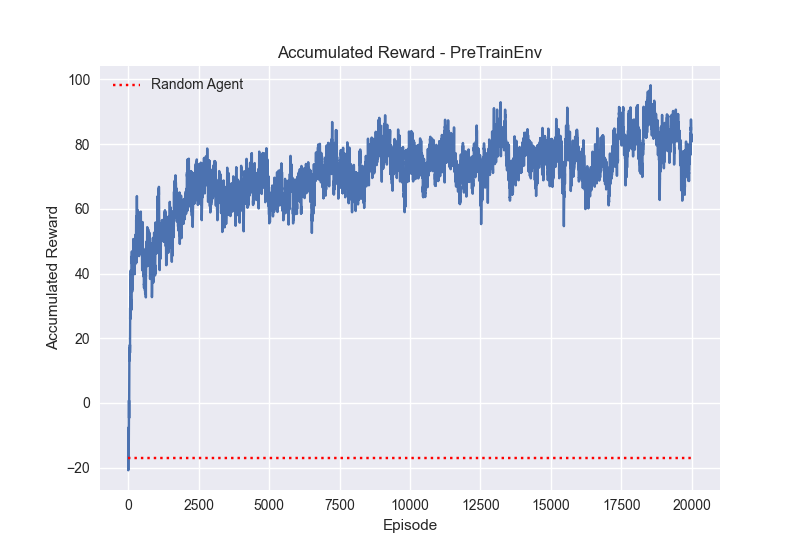
\includegraphics[width=.8\linewidth]{figuras/plot_pre_train_reward.jpg}    
  \caption{Média móvel das recompensas por episódio durante o pré-treinamento.}
  \label{fig:rew_per_ep_pretrain}
\end{figure}

\textbf{Parâmetros do Treinamento - Estágio I}
\begin{table}[H]
  \centering
  \vspace{0.5cm}
  \begin{tabular}{r|lr}
  \textbf{Parâmetro} & \textbf{Valor} \\ 
  \hline
  Número máximo de mutações por episódio ($M_{max}$) & 100 \\
  Número total de iterações ($N_{iter}$) & 2.000.000 \\
  Tamanho do batch & 200 \\
  Número máximo de repetições do mesmo aminoácido por episódio ($N_{rep}$) & 7 \\
  \end{tabular}
  \caption{Parâmetros utilizados no primeiro estágio de treinamento.}
  \label{tab:params_train_stage1}
\end{table}
